\documentclass[12pt, a4paper, twoside,  headheight=45pt, listof=totoc, bibliography=totoc]{scrreprt}
%Settings
\usepackage[T1]{fontenc}
\usepackage[utf8]{inputenc}
\usepackage[english]{babel}
\usepackage[breaklinks, hidelinks]{hyperref}
\usepackage{graphicx}
\graphicspath{{figures/}}
\usepackage{caption}
\usepackage{subcaption}
\usepackage{romannum}
\usepackage{blindtext}
\usepackage{amsmath}
\usepackage{amssymb}
\usepackage{xfrac}
\usepackage{url}
\usepackage{multirow}
\usepackage{float}
\usepackage{csquotes}
\usepackage{lscape}
\usepackage{color, soul}
\usepackage{blindtext}
\usepackage{bytefield}
\usepackage{pgfplots}
\usepackage[simplified]{pgf-umlcd}
\usepackage{tabularx}

\usepgfplotslibrary{dateplot, statistics}
\pgfplotsset{compat = newest}

\usepackage[acronym,nopostdot,nonumberlist,nogroupskip]{glossaries}
\renewcommand{\glsnamefont}[1]{\textbf{#1}}
\setlength\LTleft{0pt}
\setlength\LTright{0pt}
\setlength\glsdescwidth{0.8\hsize}
\glstoctrue
\makeglossaries
\newacronym{uml}{UML}{\textbf{U}nified \textbf{M}odeling \textbf{L}anguage}

\renewcommand {\umlfillcolor}{white}
\renewcommand {\umldrawcolor}{black}

%Font
\usepackage{lmodern}
\setkomafont{chapter}{\Large}
\setkomafont{section}{\fontsize{16pt}{16pt}}
\setkomafont{subsection}{\fontsize{14pt}{14pt}}
\usepackage{courier}
\setkomafont{caption}{\fontsize{12pt}{12pt}\bfseries}
\setkomafont{captionlabel}{\fontsize{12pt}{12pt}\bfseries}

\raggedbottom

\usepackage{enumitem}

%Settings for head and foot lines
\usepackage{scrlayer-scrpage}

%Settings for the design of a page
\usepackage[a4paper, right = 25mm , left = 25mm, top=25mm, bottom=25mm]{geometry}

\RedeclareSectionCommand[beforeskip=24pt,
afterskip=20pt]{chapter}
\RedeclareSectionCommand[beforeskip=12pt,
afterskip=8pt]{section}
\RedeclareSectionCommand[beforeskip=12pt,
afterskip=8pt]{subsection}

%Set the space between the lines
\usepackage[onehalfspacing]{setspace}

\usepackage[backend=biber, style=numeric, sorting=none]{biblatex}
\addbibresource{literature.bib}

%Footnotes numbering
\usepackage{chngcntr}
\counterwithout{footnote}{chapter}

%Advanced Settings for head and foot lines
\pagestyle{scrheadings}
%\clearscrheadfoot
\clearpairofpagestyles
\cfoot[\pagemark]{\pagemark}

%Settings for codes
\usepackage{listings}
%\renewcommand\lstlistingname{Quellcode}
%\renewcommand\lstlistlistingname{Quellcodeverzeichnis}
\usepackage{xcolor}

\definecolor{codegreen}{rgb}{0,0.6,0}
\definecolor{codegray}{rgb}{0.5,0.5,0.5}
\definecolor{codepurple}{rgb}{0.58,0,0.82}
\definecolor{backcolour}{rgb}{0.95,0.95,0.92}

\definecolor{yellow}{rgb}{1,1,0}
\definecolor{lightgreen}{rgb}{0.64,1,0.71}
\definecolor{lightred}{rgb}{1,0.7,0.71}

\lstdefinestyle{mystyle}{
    backgroundcolor=\color{backcolour},   
    commentstyle=\color{codegreen},
    keywordstyle=\color{magenta},
    numberstyle=\tiny\color{codegray},
    stringstyle=\color{codepurple},
    basicstyle=\ttfamily\footnotesize,
    breakatwhitespace=false,         
    breaklines=true,                 
    captionpos=b,                    
    keepspaces=true,                 
    numbers=left,                    
    numbersep=5pt,                  
    showspaces=false,                
    showstringspaces=false,
    showtabs=false,                  
    tabsize=2
}

\setlength{\parindent}{0pt}

\lstset{style=mystyle}



\begin{document}
\setlength{\parindent}{0pt}

\pagenumbering{Roman}
%\renewcommand{\thepage}{\roman{page}}  %for continueing after roman page count

%Titlepage
\thispagestyle{empty}

\vspace*{-1\topskip}\vspace*{-1\headsep}
%----IFS-logo--------------------------------------------------------
		\begin{figure}[!h]
			
\includegraphics[scale=.7]{ias_logo}	
		\end{figure}																	
%------------------------------------------------------------------------------
%\hrulefill

\begin{center}
\vspace*{1cm}
\textbf{\LARGE{Implementation of a Data-Driven Model Predictive
		Controller for a Self-Stabilizing Bicycle}}\\[6em]
\Large{Fürchungproject}\\[3em]
Vorgelegt an der Universität Stuttgart von \\
\textbf{\Large{Hadi Elnemr}}\\[3em]
Master of Science Informationstechnik \\ [4em]

\begin{tabular}{ll}
	\Large{Prüfern:} & \Large{Jun.-Prof. Dr.-Ing. Florian Pfaff, Prof. Dr. -Ing. Andrea Ianelli}\\
	\Large{Betreuer:} & \Large{M.Sc. Yifan Xie} \\[3em]
\end{tabular}

\textbf{5. April 2025}\\

\end{center}



\cleardoublepage

%Eidesstattliche Erklärung
\chapter*{Erklärung}
Ich erkläre, die Arbeit selbständig verfasst und bei der Erstellung dieser Arbeit die einschlägigen Bestimmungen, insbesondere zum Urheberrechtsschutz fremder Beiträge, eingehalten zu haben. Soweit meine Arbeit fremde Beiträge (z. B. Bilder, Zeichnungen, Textpassagen) enthält, erkläre ich, dass diese Beiträge als solche gekennzeichnet sind (z.B. Zitat, Quellenangabe) und ich eventuell erforderlich gewordene Zustimmungen der Urheber zur Nutzung dieser Beiträge in meiner Arbeit eingeholt habe.

\vspace*{2cm}
\begin{flushleft}
Stuttgart, den \textbf{20.05.2025}
\end{flushleft}
\begin{flushright}
\rule{45mm}{0.4pt}\\
\end{flushright}
\begin{flushright}
(...)
\end{flushright}
\cleardoublepage

\tableofcontents
\cleardoublepage

%List of figures
\listoffigures
\cleardoublepage

%List of tables
\listoftables
\cleardoublepage

%List of listings
\lstlistoflistings
\clearpage

\glsaddall
\setglossarystyle{long}
\renewcommand*{\arraystretch}{1.2}
\printglossary[type=\acronymtype]%, title=Abkürzungsverzeichnis]
\renewcommand*{\arraystretch}{1}    %set back to default


%\maketitle

%\chapter*{Abstract}
Riding a bicycle is a common activity for humans, but designing a controller to autonomously stabilise a bicycle presents significant engineering challenges.
Traditional model-based controllers, such as linear quadratic regulators (LQR) and model predictive control (MPC), require an accurate system model.
However, some parameters of a bicycle, i.e., the centre of gravity, can be difficult to determine and may fluctuate due to varying loads or additional passengers.
In this research project, a data-driven state-feedback controller is implemented to stabilise an autonomous mini-bike by solving a semidefinite program (SDP).
The method does not identify the system model of the bicycle and directly uses noisy collected data to design the controller.
Two models of the bicycle are used to test and assess the controller.
Along with the simulations, experiments on a model-scale bicycle demonstrate successful stabilisation using noisy data generated based on the system dynamics.
%\cleardoublepage

%\include{kurzfassung}
%\cleardoublepage

\cleardoublepage
\chapter*{Abstract}
Riding a bicycle is a common activity for humans, but designing a controller to autonomously stabilise a bicycle presents significant engineering challenges.
Traditional model-based controllers, such as linear quadratic regulators (LQR) and model predictive control (MPC), require an accurate system model.
However, some parameters of a bicycle, i.e., the centre of gravity, can be difficult to determine and may fluctuate due to varying loads or additional passengers.
In this research project, a data-driven state-feedback controller is implemented to stabilise an autonomous mini-bike by solving a semidefinite program (SDP).
The method does not identify the system model of the bicycle and directly uses noisy collected data to design the controller.
Two models of the bicycle are used to test and assess the controller.
Along with the simulations, experiments on a model-scale bicycle demonstrate successful stabilisation using noisy data generated based on the system dynamics.
\cleardoublepage

\pagenumbering{arabic}
%\renewcommand{\thepage}{\arabic{page}}  %for continueing after roman page count

\chapter{Introduction}

Riding a bicycle is a common activity for humans, but designing a controller to autonomously stabilize a bicycle presents significant engineering challenges.
Traditional model-based controllers, such as linear quadratic regulators (LQR) and model predictive control (MPC), require an accurate system model. 
However, some parameters of a bicycle, i.e., the center of gravity, can be difficult to determine and may fluctuate due to varying loads or additional passengers. 
In this project, we aim to design and implement a data-driven MPC controller to stabilize an autonomous mini bike. 
The method does not identify the system model of the bike and directly uses the collected data to design the controller. The goal is to stabilize the bike at a constant speed and the bike does not fall down. 
Besides, we aim to keep both the lean angle and steering angle within defined safe limits for safety.


%\section{Literature Review}
%Hello \cite{grimmeisen2022case}
%\gls{uml}
%% Bicycle Modeling Literature Review
\section{Bicycle Modeling}

	The modeling of autonomous bicycles is a fundamental step towards designing controllers capable of maintaining balance and ensuring stable motion. Due to the inherent instability and nonlinearity of bicycles, developing accurate mathematical models has been a significant focus in recent research. Various approaches have been proposed to model the dynamics of bicycles, with key methodologies including linear-parameter-varying (LPV) models, kinetic models, and state-space representations.
	
	\subsection{Linear-Parameter-Varying (LPV) Models}
	One of the primary methods used in bicycle modeling is the Linear-Parameter-Varying (LPV) approach, which accounts for variations in parameters, such as velocity, that affect the stability of the bicycle. The LPV framework is particularly useful when the bicycle's speed is subject to change, as it enables the controller to adapt to varying conditions.
	
	Cerone et al. (2010) proposed an LPV-based stabilization method for riderless bicycles, which uses a parameter-varying approach to handle the dynamic changes in speed. The study demonstrated that stability can be maintained between two specific speeds by discretizing the continuous-time system, thereby addressing the nonlinearity inherent in the bicycle dynamics\cite{cerone2010}.
	
	\subsection{Kinetic and Dynamic Models}
	In contrast to LPV models, kinetic models focus on the fundamental forces and motions of the bicycle, including the relation between lean angle, steering angle, and speed. Tapken et al. (2018) presented a comprehensive study on modeling the kinetic and dynamic aspects of bicycles, employing tools such as CAD modeling and Simscape Multibody to simulate the motion accurately \cite{tapken2018}.
	
	The kinetic model is essential when dealing with physical prototypes, as it directly links the control inputs to the physical response of the bicycle. The combination of kinetic modeling with state-space representations allows for a more comprehensive analysis, particularly when integrating control algorithms such as LQR or PID controllers.
	
	\subsection{Comparative Analysis of Models}
	Persson et al. (2021) conducted a comparative analysis of various control models applied to autonomous bicycles. The study highlighted the advantages of using LPV models for systems with varying speeds, while kinetic models proved effective for low-speed stability. This comparison underlines the importance of model selection based on the specific application requirements \cite{persson2021}.
	
	In conclusion, accurate modeling of autonomous bicycles requires a balance between capturing the system's dynamic complexity and maintaining computational efficiency. While LPV models offer flexibility in handling speed variations, kinetic models are indispensable for physical implementations and control integration.

%% Bicycle Control Literature Review
\section{Bicycle Control}

	Controlling autonomous bicycles poses significant challenges due to their inherently unstable dynamics and the need to maintain balance while steering. Effective control strategies must account for disturbances, speed variations, and the nonlinear nature of bicycle motion. Over the years, various control methods have been proposed, ranging from classical techniques to more advanced model-based and data-driven approaches.
	
	\subsection{Traditional Control Methods}
	Classical control techniques such as Proportional-Integral-Derivative (PID) control and Linear Quadratic Regulator (LQR) control have been extensively applied to bicycle stabilization. The PID controller is widely used for velocity and lean angle control due to its simplicity and effectiveness. However, it may not guarantee robust stability, particularly in dynamically changing conditions.
	
	The LQR controller, on the other hand, optimizes a quadratic cost function, balancing the trade-off between control effort and system stability. Persson et al. (2021) demonstrated that LQR provides smoother stabilization compared to PID, especially when the bicycle model is linearized\cite{persson2021}. Despite its advantages, LQR assumes a known and accurate model, limiting its applicability in scenarios with model uncertainties.
	
	\subsection{Advanced Control Techniques}
	To address the limitations of traditional methods, advanced control strategies have been developed. Andersson et al. (2019) proposed a loop-shaping method to stabilize riderless bicycles. This method focuses on shaping the open-loop transfer function to ensure robust stability across varying speeds \cite{andersson2019}.
	
	State-feedback control has also gained attention as it directly incorporates the measured states into the control law. Turnwald et al. (2019) demonstrated a successful implementation of state-feedback control in an autonomous bicycle, achieving reliable balance even under external disturbances \cite{turnwald2019}.
	
	\subsection{Comparative Analysis of Control Strategies}
	A comparative study by Yu et al. (2018) investigated the effectiveness of steering control at low speeds, highlighting that traditional PID control is less effective when the bicycle operates near its tipping point. In contrast, the adaptive state-feedback method provided consistent performance across various speed conditions \cite{yu2018}.
	
	\subsection{Experimental Validation and Results}
	Experimental implementations revealed that while traditional methods can stabilize the bicycle at fixed speeds, advanced methods such as loop shaping and state-feedback control provide more flexibility. These methods better handle model uncertainties and external disturbances, which are crucial for autonomous operation.
	
	In summary, bicycle control strategies have evolved from simple PID-based methods to more robust and adaptive approaches. Advanced techniques such as LQR, state-feedback, and loop shaping offer improved performance, particularly when dealing with speed variations and external disturbances.

%% Data-Driven Control Methods Literature Review
\section{Data-Driven Control Methods}

	The increasing complexity and dynamic nature of autonomous systems, such as self-balancing bicycles, have led to the development of data-driven control methods. These methods bypass the need for precise system modeling by directly utilising measurement data to infer control actions. Data-driven approaches are particularly valuable when model inaccuracies or environmental disturbances are significant.
	
	\subsection{Data-Driven Model Predictive Control (MPC)}
	Model Predictive Control (MPC) is a widely used approach for controlling systems with constraints. Traditional MPC relies on accurate mathematical models to predict system behavior. However, data-driven MPC approaches directly utilize input-output data to predict future states, thus mitigating modeling errors.
	
	One notable approach is the \textbf{Data-Driven Min-Max MPC}, which aims to robustly stabilize the system while minimizing the worst-case cost. Xie et al. (2024) proposed a robust min-max MPC framework that incorporates noisy input-state data, formulating the control problem as a semi-definite program (SDP). This method guarantees robust stability and constraint satisfaction while reducing conservatism compared to traditional data-driven MPC approaches \cite{xie2024}.
	
	Adaptive data-driven MPC has also been proposed to further improve performance by continuously integrating new data. This adaptive strategy reduces model uncertainty over time, leading to more precise control. The combination of min-max optimization and online adaptation provides enhanced robustness, especially in systems with time-varying parameters \cite{xie2024}.
	
	\subsection{Comparative Analysis of Data-Driven MPC Methods}
	A significant advantage of data-driven MPC is its ability to handle uncertainties without requiring an explicit system model. Compared to classical model-based MPC, data-driven methods are more adaptable when the system's dynamics change. Additionally, the use of online data in adaptive MPC helps reduce conservatism, achieving better closed-loop performance \cite{xie2024}.
	
	Yu et al. (2018) demonstrated that data-driven steering control techniques could maintain stability at low speeds, where conventional control strategies often fail. This highlights the practicality of data-driven control in real-world applications \cite{yu2018}.
	
	\subsection{Experimental Validation and Results}
	Experimental studies have shown that data-driven MPC can effectively stabilize bicycles, even when the underlying dynamic model is not accurately known. Adaptive schemes have demonstrated improved performance over static data-driven methods by continuously refining the control law based on new data \cite{xie2024}.
	
	In conclusion, data-driven control methods offer a promising approach to managing the inherent uncertainties in autonomous bicycles. By leveraging real-time data, these methods can adapt to changing conditions and maintain robust performance, making them superior to purely model-based techniques in many scenarios.


\section{History of IST Bike}

\section{WHEELTEC MiniBike}
In this research project, a self-balancing mini-bike developed by \textbf{WHEELTEC} was utilized as the experimental platform. The primary goal of the project is to implement a data-driven State-Feedback Controller for stabilizing the bike. The mini-bike is equipped with various sensors and actuators to enable control and data acquisition.

	%% Mini-Bike Overview Section for Thesis
	
	\subsection{Mini-Bike Structure and Components}
	The mini-bike is based on the \textbf{WHEELTEC Z100 Servo Self-Balancing Bicycle} in Figure \ref{fig:minibike}. It features an STM32F103C8T6 microcontroller as the primary control unit, which integrates differenct sensors and motor control circuits to achieve stabilization. The bike has the following key components:
	\begin{itemize}
		\item \textbf{Gyroscope (MPU6050)}: Provides angular velocity and acceleration data necessary for balancing the bike.
		\item \textbf{Motor and Encoder}: The rear wheel motor is driven by an H-bridge circuit (AT8236), while the encoder measures rotational speed and position, enabling closed-loop control.
		\item \textbf{Servo Motor}: Controls the steering mechanism, essential for maintaining balance during motion.
		\item \textbf{Power Supply}: Powered by a 2S lithium-ion battery, maintaining an optimal voltage range of 7 to 12 volts.
		\item \textbf{Bluetooth Module}: Allows remote control and data transmission via the MiniBalance mobile app.
	\end{itemize}
	
	\subsection{Balancing and Control Mechanism}
	The bike achieves self-balancing through controlling the steering angle. This is done through a controller computed using \textbf{Linear Quadratic Regulator (LQR)} combined with a \textbf{PID controller}. The LQR calculates optimal control inputs based on the state feedback to minimize the cost function, while the PID controller fine-tunes the steering speed by adjusting the PWM signals to the servo motor.
	
	The system's balance is continuously monitored through the gyroscope, which provides real-time data on tilt angles and angular velocities. These values are processed by the microcontroller to compute the necessary adjustments to the rear wheel and steering servo to maintain balance.
	
	\subsection{Data Collection and Experimental Setup}
	Data from the bike can be collected using the \textbf{USART1} for transmission to a host computer and \textbf{USART3} for Bluetooth communication. The mobile application displays data such as tilt angles, angular velocity, and PWM values, allowing for parameter adjustments during testing.
	
	\subsection{Operation and Control Interface}
	The mini-bike can be operated using a mobile application that connects via Bluetooth. The app allows the user to control the bike's direction and view live data for diagnostic purposes. Additionally, a waveform display can be accessed via a PC for more detailed analysis.
	
	\subsection{Challenges and Adjustments}
	One of the challenges encountered was the adjustment of the balance midpoint, which can be fine-tuned using potentiometers located on the main board. These potentiometers adjust the balance point without needing to modify the control algorithm directly, which is particularly useful for maintaining stability under varying conditions.
	
	In summary, the WHEELTEC mini-bike served as an experimental platform for the implementation and testing of the data-driven feedback controller, providing a practical application for a stabilisation system.
	
	\begin{figure}
		\centering
		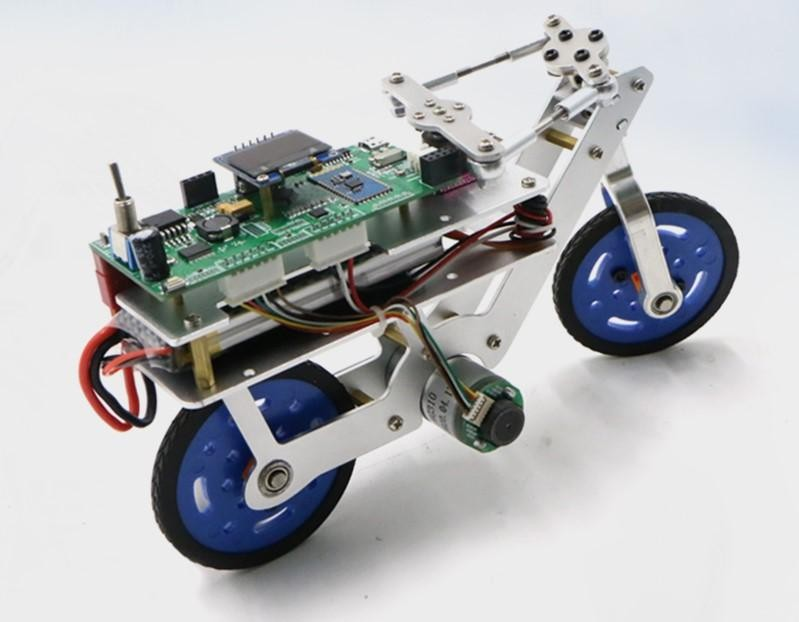
\includegraphics[width=0.7\linewidth]{figures/minibike/minibike}
		\caption{A picture for the MiniBike used in the experiments.}
		\label{fig:minibike}
	\end{figure}





\section{Structure of thesis}
This thesis is structured as follows:
Chapter 1 provides an introduction, including the background, motivation, and objectives of the research.
Chapter 2 discusses the theoretical foundations, focusing on Model Predictive Control (MPC) and related concepts.
Chapter 3 describes the simulation setup and the implementation of the data-driven MPC approach.
Chapter 4 presents the experimental results, including the setup and data collection from the mini-bike.
Chapter 5 concludes the report and discusses future work.





%%%%%%%%%%%%%%%%%%%%%%%%%%%%%%%%%%%
    2,3 Bike Institute Morlock: (Fill in relevant information)

1.1 Liter: (Fill in relevant information)

1.2 History Institute Bike: (Fill in relevant information)

1.3 Structure of Thesis:
This thesis is structured as follows:

Chapter 1 provides an introduction, including the background, motivation, and objectives of the research.

Chapter 2 discusses the theoretical foundations, focusing on Model Predictive Control (MPC) and related concepts.

Chapter 3 describes the simulation setup and the implementation of the data-driven MPC approach.

Chapter 4 presents the experimental results, including the setup and data collection from the mini-bike.

Chapter 5 concludes the report and discusses future work.

Motivation:
Designing a controller for an autonomous bicycle presents significant engineering challenges, especially when the model parameters, such as the center of gravity, fluctuate due to varying loads. Traditional model-based controllers require an accurate system model, which may be difficult to determine. This research explores the use of a data-driven MPC controller to stabilize a mini-bike, bypassing the need for a precise system model and instead using collected data to inform control decisions. The goal is to stabilize the bike at a constant speed while keeping both the lean angle and steering angle within defined safe limits.
Theory
Main Results

The Model Predictive Control (MPC) approach used in this research is a type of state-feedback controller. In the context of bicycle stabilization, the MPC controller uses real-time data to predict future states of the system and adjusts the inputs accordingly to minimize a cost function. This approach allows the bike to maintain stability and stay within safe operating limits without relying on a detailed system model.

State-feedback Controller:
A state-feedback controller is designed by using the measured states of the system (e.g., lean angle, steering angle) to compute the control input (e.g., steering angle) that stabilizes the bike.

MPC Theory:
The data-driven MPC uses historical data to estimate system parameters and define the constraints and objective function in the optimization problem. The key innovation is the use of real-time data to adapt the control strategy without relying on an explicit system model.

Derivation of Main Results:

The key concept behind the data-driven MPC is to optimize the control input at each time step based on the current state and past data, adjusting for uncertainties and external disturbances like changes in the load or rider position.

Simulation
State-feedback Controller

The simulation setup includes the implementation of a state-feedback controller based on the equations derived in the previous section. The bike model used for simulation is a simplified version of a front-steered bicycle, where key states like the lean angle and steering angle are tracked.
MPC Implementation

Data-driven MPC: This section discusses the application of the data-driven approach to stabilize the bike. The controller’s performance is evaluated by comparing it to a traditional MPC setup, where the system model is known.

Comparison (Discussion):
The results of the simulations are compared based on the control performance, including stabilization time, error rates, and the ability to handle disturbances. The comparison highlights the advantages and limitations of the data-driven MPC approach compared to traditional methods.

Experiment
Implementation of the State-feedback Controller

This section details the implementation of the state-feedback controller on the real mini-bike, including:

The STM32 microcontroller code

Data collection for both open-loop and closed-loop experiments

Implementation of Data-driven MPC

The data-driven MPC controller is implemented on the mini-bike using the STM32 microcontroller, integrating the appropriate solver for the Semi-Definite Program (SDP). The results from the real-world experiments are compared to the simulation results to validate the effectiveness of the data-driven approach.
Results
Simulations

The results of the simulations are presented, including graphs and metrics for:

Stabilization performance

Lean angle and steering angle control

Comparison of data-driven MPC vs. traditional MPC

Implementation and Experimental Setup

The experimental setup for testing the self-stabilizing bike is described in detail:

Hardware components (e.g., STM32 microcontroller, sensors, actuators)

Experimental setup for real bike testing

Data collection methods (e.g., sensor readings, control inputs)

Results from the Experiment

State-feedback Controller Performance:
A comparison of the performance of the state-feedback controller when implemented on the real bike is presented, including any challenges encountered during implementation.

Data-driven MPC Performance:
The performance of the data-driven MPC is evaluated based on its ability to stabilize the bike and maintain control over the lean and steering angles under different conditions.

Conclusion

In conclusion, this research presents a data-driven MPC approach for stabilizing a self-balancing mini-bike. The results from both simulations and real-world experiments demonstrate the effectiveness of the data-driven approach compared to traditional MPC methods. Future work may include experimenting with the rear-steered mode of the bike (optional) and further improving the robustness of the controller in dynamic environments.

\chapter{Literature Review - Bicycle Modeling and Control}
%\section{Section1}
\cleardoublepage


\printbibliography
\end{document}